\documentclass[a0,portrait]{a0poster}

\usepackage{multicol}
\columnsep=100pt
\columnseprule=3pt

\usepackage[svgnames]{xcolor}

\usepackage{times}
\usepackage{palatino}
\usepackage[none]{hyphenat}
\usepackage{graphicx}
\graphicspath{{figures/}}
\usepackage{booktabs}
\usepackage[font=small,labelfont=bf]{caption}
\usepackage{amsfonts, amsmath, amsthm, amssymb}
\usepackage{wrapfig}
\usepackage{lipsum,adjustbox}
\usepackage[absolute,overlay]{textpos}
\usepackage{multirow}
\usepackage{titlesec}
\usepackage[inline]{enumitem}
\usepackage{url}
\usepackage{tikz,pgfplots,pgfplotstable}
\usepackage{tikz-dependency}
\usetikzlibrary{arrows.meta}
\captionsetup{labelformat=empty}

\begin{document}

\begin{center}
	\veryHuge \color{NavyBlue} \textbf{Universal Dependency Parsing \\
	with a General Transition-Based DAG Parser}
\end{center}
\begin{minipage}[b]{0.57\linewidth}
\LARGE \textbf{Daniel Hershcovich}\textsuperscript{1,2} \&
	   \textbf{Omri Abend}\textsuperscript{2} \&
	   \textbf{Ari Rappoport}\textsuperscript{2} \\[0.5cm]
\large $^1$The Edmond and Lily Safra Center for Brain Sciences \\
  $^2$School of Computer Science and Engineering
  \setlength{\columnseprule}{0pt}
  \setlength\multicolsep{-20pt}
  \begin{multicols}{2}
  The Hebrew University of Jerusalem \\
  \texttt{\{danielh,oabend,arir\}@cs.huji.ac.il}
  \end{multicols}
\end{minipage}
\hfill
\begin{minipage}[b]{.1\linewidth}

\includegraphics[width=\linewidth]{elsc_logo.png}
\end{minipage}
\begin{minipage}[b]{.18\linewidth}

\includegraphics[width=\linewidth]{huji_banner.png}

\includegraphics[width=1.04\linewidth]{cse_banner.jpg}
\end{minipage}
\begin{minipage}[b]{.07\linewidth}

\includegraphics[width=\linewidth]{huji_logo.jpg}
\end{minipage}

\vspace{1cm}
\titlespacing*{\section}{0pt}{8mm}{5mm}

%----------------------------------------------------------------------------------------


\begin{adjustbox}{margin=5mm,frame,minipage=.75\linewidth,center}
\Large\color{Navy}
Learning to parse \textbf{enhanced dependencies} jointly with the basic Universal Dependency Parsing task.
\end{adjustbox}


\begin{multicols}{2}


\color{Black}

\begin{itemize}[labelsep=1em]
{\color{Indigo} \item[\textbf{UCCA}:] Intuitive, cross-lingual, and modular semantic representation.
    \textit{Primary edges} form a tree. \textit{Remote edges} (dashed) allow reentrancy,
    creating a directed acyclic graph \cite{abend2013universal}.}
{\color{DarkBlue} \item[\textbf{UD}:] Cross-lingual syntactic bilexical tree.
    Encodes syntactic relations between words \cite{nivre2016universal}. \\
    \textbf{UD$^{++}$} (Enhanced++ UD) adds and augments edges, creating a bilexical DAG
    \cite{SCHUSTER16.779}.}
\end{itemize}

\begin{minipage}{.45\columnwidth}
  \color{Indigo}
  \begin{center}
  \scalebox{.6}{
    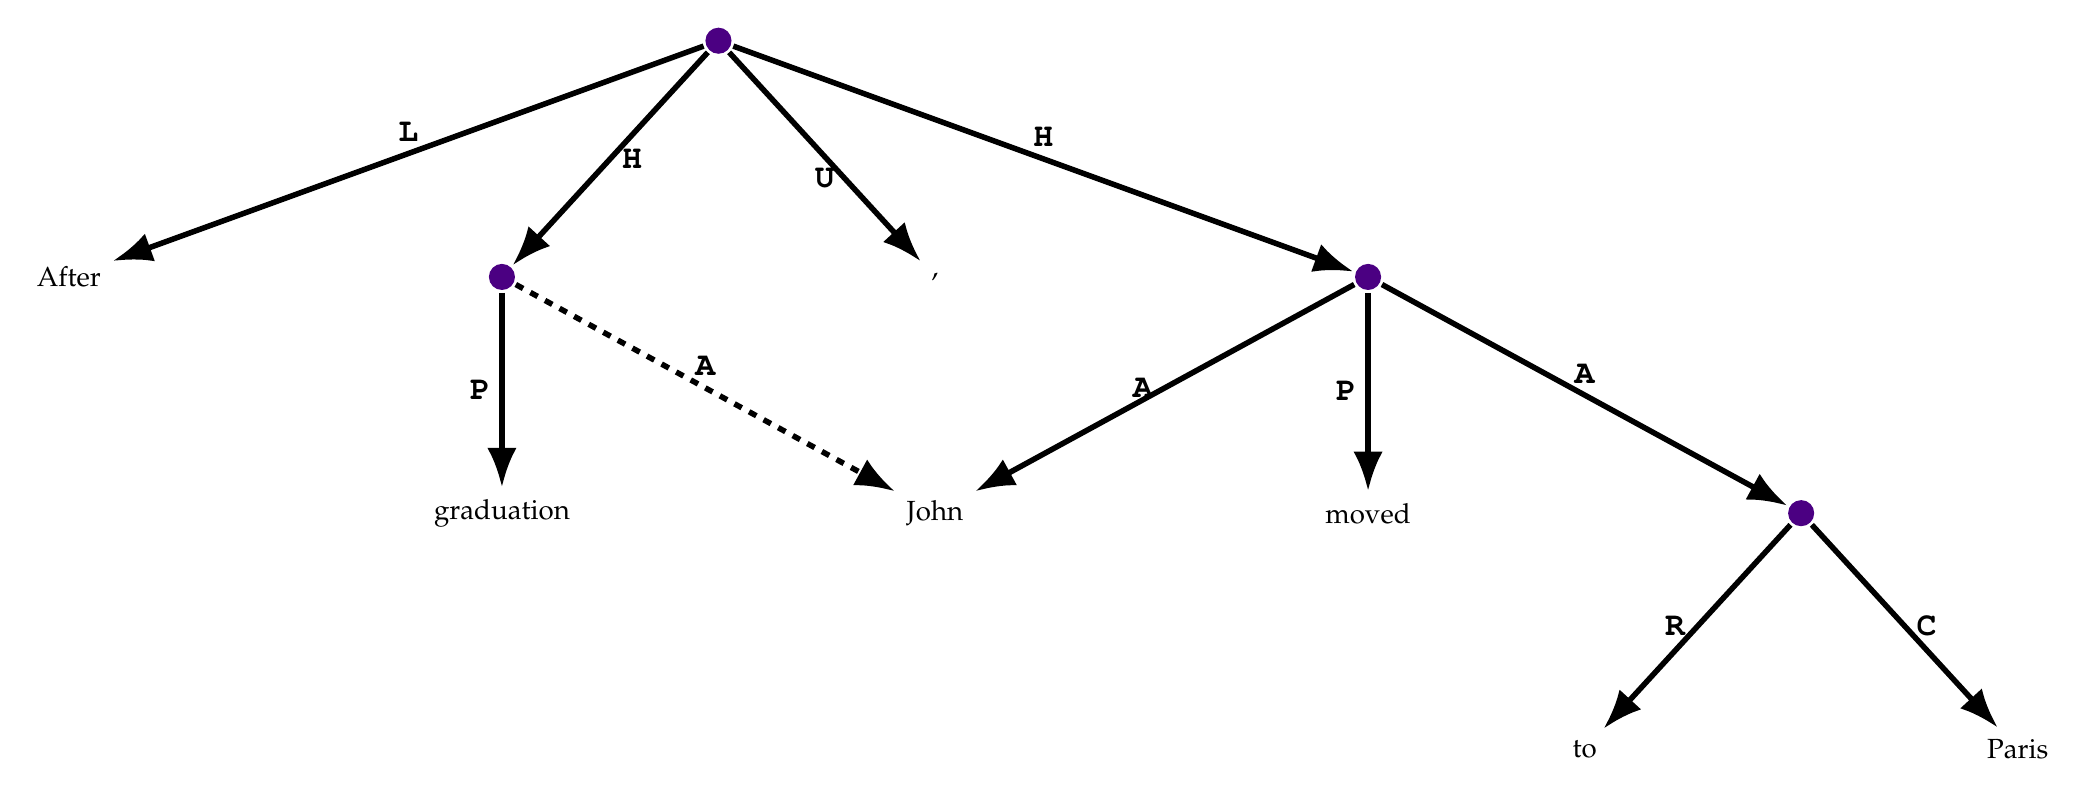
\begin{tikzpicture}[level distance=3cm, sibling distance=55mm, -{Latex[length=5mm]}, line width=2pt,
        every node/.append style={font=\large\bf\ttfamily},
        every circle node/.append style={fill=Indigo}]
      \tikzstyle{word} = [font=\rmfamily,color=black]
      \node (ROOT) [circle] {}
        child {node (After) [word] {After} edge from parent node[above] {L}}
        child {node (graduation) [circle] {}
        {
          child {node [word] {graduation} edge from parent node[left] {P}}
        } edge from parent node[right] {H} }
        child {node [word] {,} edge from parent node[below] {U}}
        child {node (moved) [circle] {}
        {
          child {node (John) [word] {John} edge from parent node[left] {A}}
          child {node [word] {moved} edge from parent node[left] {P}}
          child {node [circle] {}
          {
            child {node [word] {to} edge from parent node[left] {R}}
            child {node [word] {Paris} edge from parent node[right] {C}}
          } edge from parent node[above] {A} }
        } edge from parent node[above] {H} }
        ;
      \draw[dashed,-{Latex[length=5mm]}] (graduation) to node [above] {A} (John);
    \end{tikzpicture}
  }
  \captionof{figure}{\color{Indigo} Universal Conceptual Cognitive Annotation (UCCA).}
  \end{center}
\end{minipage}
\begin{minipage}{.55\columnwidth}
    \begin{center}
    \begin{dependency}[edge style={-{Latex[length=4mm]}, color=DarkBlue, line width=2pt},
        text only label, label style={above, color=DarkBlue, font=\bf\ttfamily}, font=\small]
    \begin{deptext}[column sep=.8em,ampersand replacement=\^, color=DarkBlue]
    After \^ graduation \^ , \^ John \^ moved \^ to \^ Paris \\
    \end{deptext}
        \depedge[edge unit distance=1em]{2}{1}{case}
        \depedge[edge unit distance=1em]{4}{3}{punct}
        \depedge[edge unit distance=1em, edge start x offset=-4mm]{5}{4}{nsubj}
        \depedge[edge unit distance=1em, edge end x offset=-3mm]{2}{5}{obl}
        \depedge[edge unit distance=1em]{7}{6}{case}
        \deproot[edge unit distance=1em]{5}{root}
        \depedge[edge unit distance=1.5em, edge start x offset=1mm]{5}{7}{obl}
    \end{dependency}
  \captionof{figure}{\color{DarkBlue} Universal Dependencies (UD).}
  \end{center}
\end{minipage}

\vspace{5mm}

\hrule


\section*{TUPA: A Transition-Based DAG Parser}

We extend TUPA, a general DAG parser,
which has been proposed as a UCCA parser \cite{hershcovich2017a}. \\
It is a transition-based parser supporting reentrancy, discontinuity and non-terminal nodes.

\scalebox{.9}{
\begin{minipage}{.55\columnwidth}
	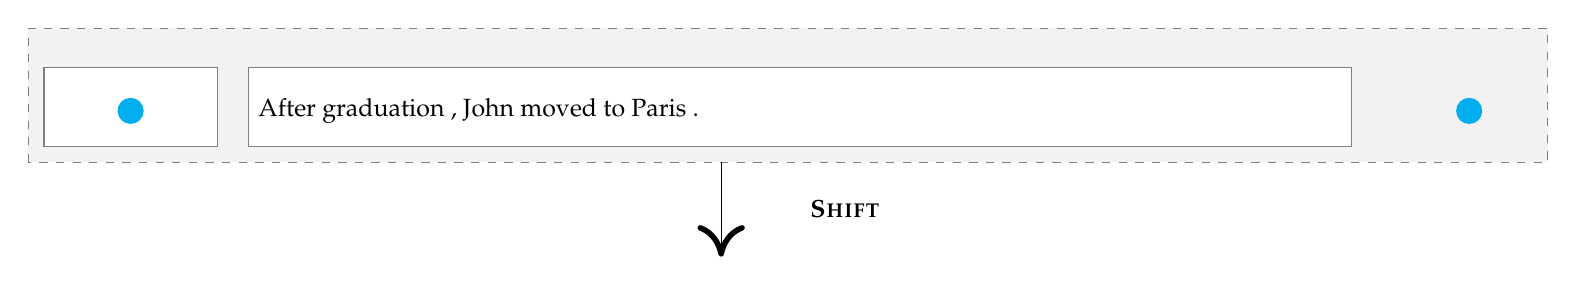
\begin{tikzpicture}[level distance=15mm, sibling distance=4cm, font=\small]
	\draw[color=gray,dashed,fill=lightgray!20] (.2,-.2) rectangle (19.5,1.5);
	\draw[color=gray,fill=white] (.4,0) rectangle (2.6,1);
	\node[fill=cyan, circle] at (1.5,.45) {};
	\draw[color=gray,fill=white] (3,0) rectangle (17,1);
	\node[anchor=west] at (3,.45) {After graduation , John moved to Paris .};
	\node[fill=cyan, circle] at (18.5,.45) {};
	\node[anchor=west] at (10,-.8) {\bf\small\textsc{Shift}};
	\draw[arrows={->[line width=2pt,length=4mm,width=6mm]}] (9,-.2) -- (9,-1.4);
	\end{tikzpicture}
	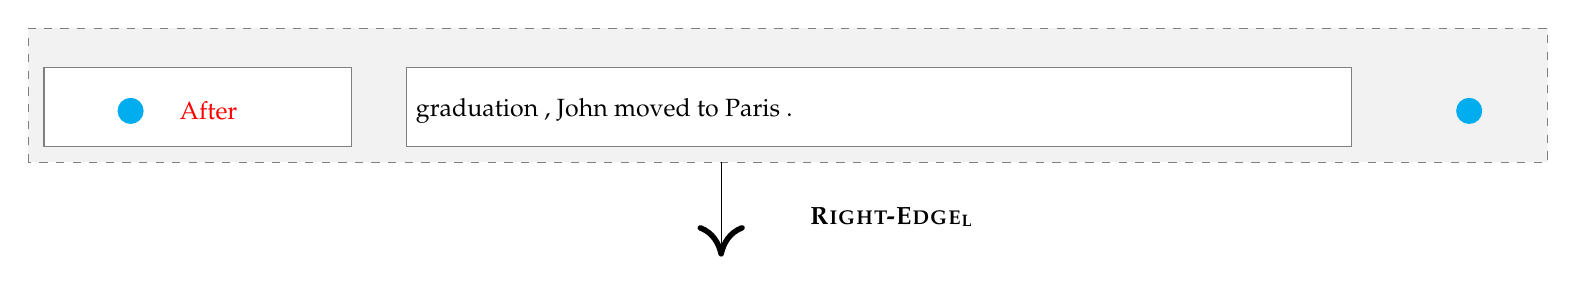
\begin{tikzpicture}[level distance=15mm, sibling distance=4cm, font=\small]
	\draw[color=gray,dashed,fill=lightgray!20] (.2,-.2) rectangle (19.5,1.5);
	\draw[color=gray,fill=white] (.4,0) rectangle (4.3,1);
	\node[fill=cyan, circle] at (1.5,.45) {};
	\node[color=red,anchor=west] at (2,.45) {After};
	\draw[color=gray,fill=white] (5,0) rectangle (17,1);
	\node[anchor=west] at (5,.45) {graduation , John moved to Paris .};
	\node[fill=cyan, circle] at (18.5,.45) {};
	\node[anchor=west] at (10,-.9) {\bf\small\textsc{Right-Edge\textsubscript L}};
	\draw[arrows={->[line width=2pt,length=4mm,width=6mm]}] (9,-.2) -- (9,-1.4);
	\end{tikzpicture}
	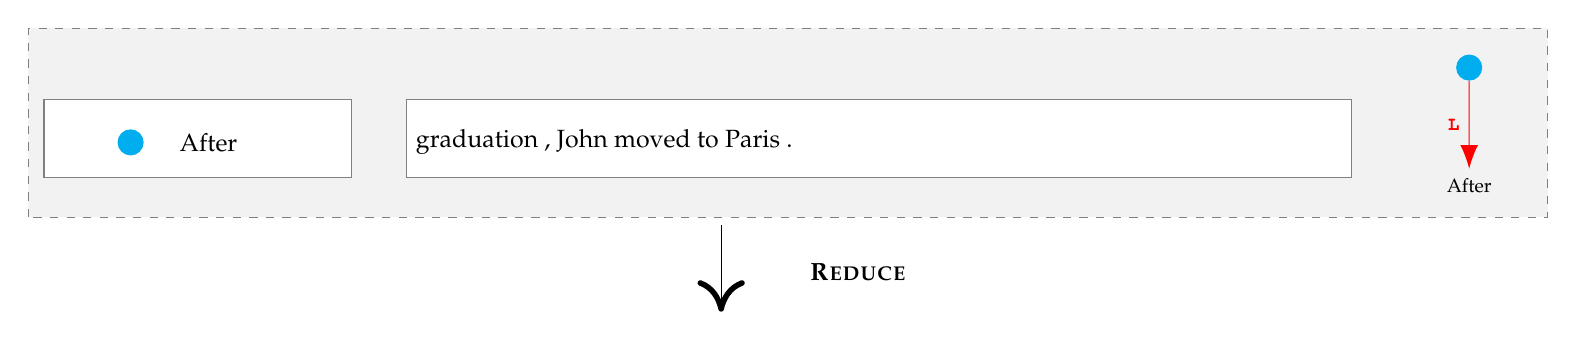
\begin{tikzpicture}[level distance=15mm, sibling distance=4cm, font=\small, -{Latex[length=3mm]}]
	\draw[color=gray,dashed,fill=lightgray!20] (.2,-.5) rectangle (19.5,1.9);
	\draw[color=gray,fill=white] (.4,0) rectangle (4.3,1);
	\node[fill=cyan, circle] at (1.5,.45) {};
	\node[anchor=west] at (2,.45) {After};
	\draw[color=gray,fill=white] (5,0) rectangle (17,1);
	\node[anchor=west] at (5,.45) {graduation , John moved to Paris .};
	\node[fill=cyan, circle] at (18.5,1.4) {}
	  child {node[font=\scriptsize] {After} edge from parent [red] node[font=\scriptsize\bf\ttfamily,left] {L}};
	\node[anchor=west] at (10,-1.2) {\bf\small\textsc{Reduce}};
	\draw[arrows={->[line width=2pt,length=4mm,width=6mm]}] (9,-.6) -- (9,-1.7);
	\end{tikzpicture}
	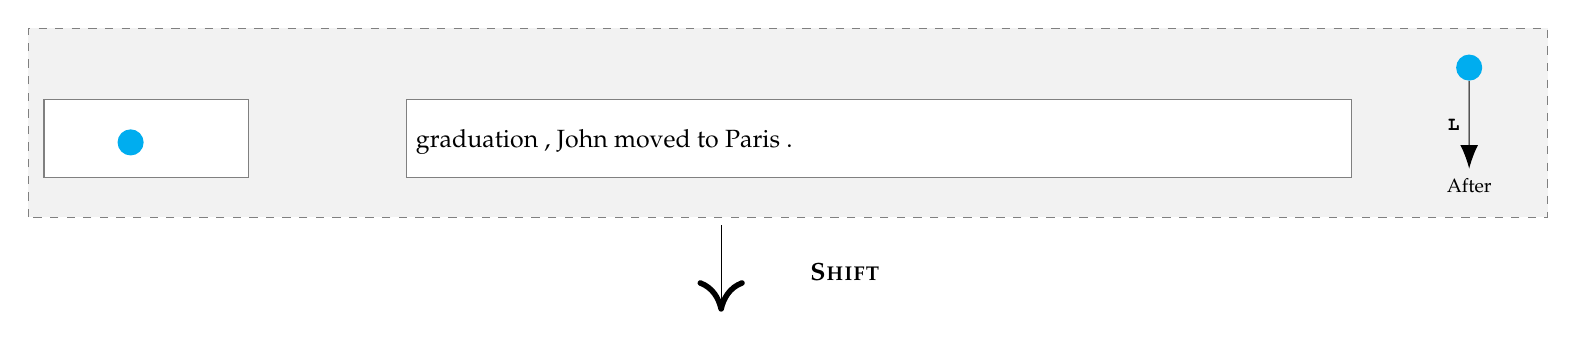
\begin{tikzpicture}[level distance=15mm, sibling distance=4cm, font=\small, -{Latex[length=3mm]}]
	\draw[color=gray,dashed,fill=lightgray!20] (.2,-.5) rectangle (19.5,1.9);
	\draw[color=gray,fill=white] (.4,0) rectangle (3,1);
	\node[fill=cyan, circle] at (1.5,.45) {};
	\draw[color=gray,fill=white] (5,0) rectangle (17,1);
	\node[anchor=west] at (5,.45) {graduation , John moved to Paris .};
	\node[fill=cyan, circle] at (18.5,1.4) {}
	  child {node[font=\scriptsize] {After} edge from parent node[font=\scriptsize\bf\ttfamily,left] {L}};
	\node[anchor=west] at (10,-1.2) {\bf\small\textsc{Shift}};
	\draw[arrows={->[line width=2pt,length=4mm,width=6mm]}] (9,-.6) -- (9,-1.7);
	\end{tikzpicture}
	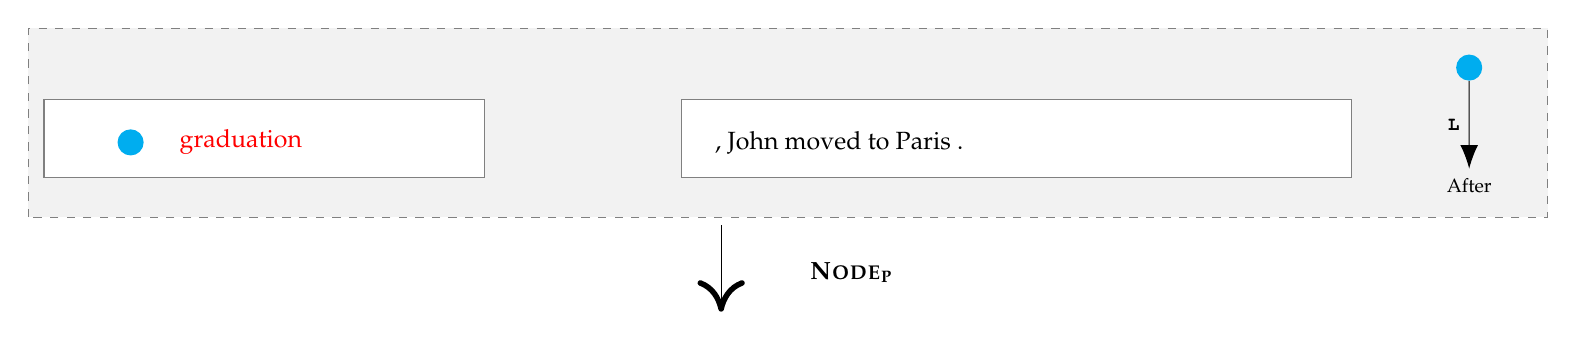
\begin{tikzpicture}[level distance=15mm, sibling distance=4cm, font=\small, -{Latex[length=3mm]}]
	\draw[color=gray,dashed,fill=lightgray!20] (.2,-.5) rectangle (19.5,1.9);
	\draw[color=gray,fill=white] (.4,0) rectangle (6,1);
	\node[fill=cyan, circle] at (1.5,.45) {};
	\node[color=red,anchor=west] at (2,.45) {graduation};
	\draw[color=gray,fill=white] (8.5,0) rectangle (17,1);
	\node[anchor=west] at (8.8,.45) {, John moved to Paris .};
	\node[fill=cyan, circle] at (18.5,1.4) {}
	  child {node[font=\scriptsize] {After} edge from parent node[font=\scriptsize\bf\ttfamily,left] {L}};
	\node[anchor=west] at (10,-1.2) {\bf\small\textsc{Node\textsubscript P}};
	\draw[arrows={->[line width=2pt,length=4mm,width=6mm]}] (9,-.6) -- (9,-1.7);
	\end{tikzpicture}
	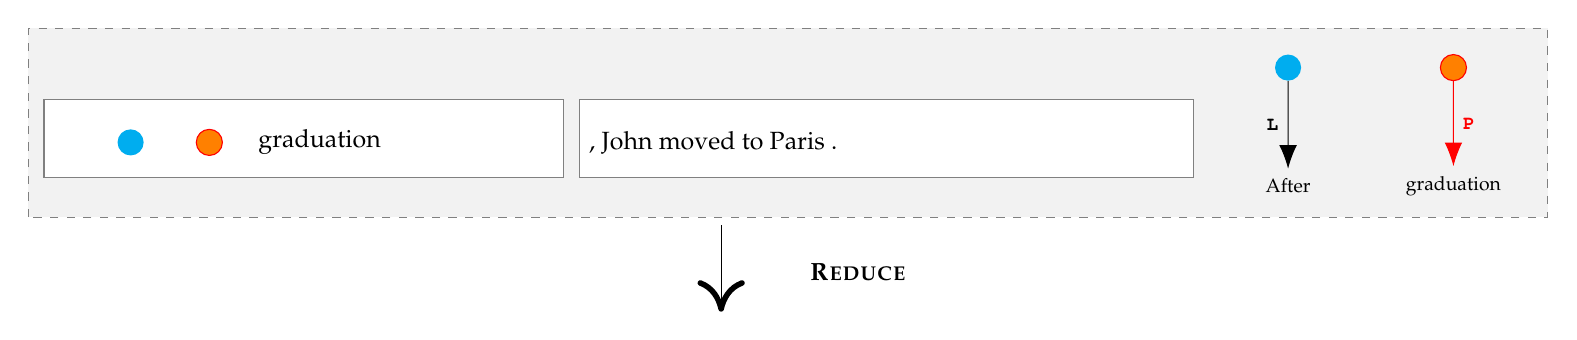
\begin{tikzpicture}[level distance=15mm, sibling distance=4cm, font=\small, -{Latex[length=3mm]}]
	\draw[color=gray,dashed,fill=lightgray!20] (.2,-.5) rectangle (19.5,1.9);
	\draw[color=gray,fill=white] (.4,0) rectangle (7,1);
	\node[fill=cyan, circle] at (1.5,.45) {};
	\node[fill=orange, draw=red, circle] at (2.5,.45) {};
	\node[anchor=west] at (3,.45) {graduation};
	\draw[color=gray,fill=white] (7.2,0) rectangle (15,1);
	\node[anchor=west] at (7.2,.45) {, John moved to Paris .};
	\node[fill=cyan, circle] at (16.2,1.4) {}
	  child {node[font=\scriptsize] {After} edge from parent node[font=\scriptsize\bf\ttfamily,left] {L}};
	\node[fill=orange, draw=red, circle] at (18.3,1.4) {}
	  child {node[font=\scriptsize] {graduation} edge from parent [red] node[font=\scriptsize\bf\ttfamily,right] {P}};
	\node[anchor=west] at (10,-1.2) {\bf\small\textsc{Reduce}};
	\draw[arrows={->[line width=2pt,length=4mm,width=6mm]}] (9,-.6) -- (9,-1.7);
	\end{tikzpicture}
\end{minipage}
\hspace{1cm}
\begin{minipage}{.4\columnwidth}
	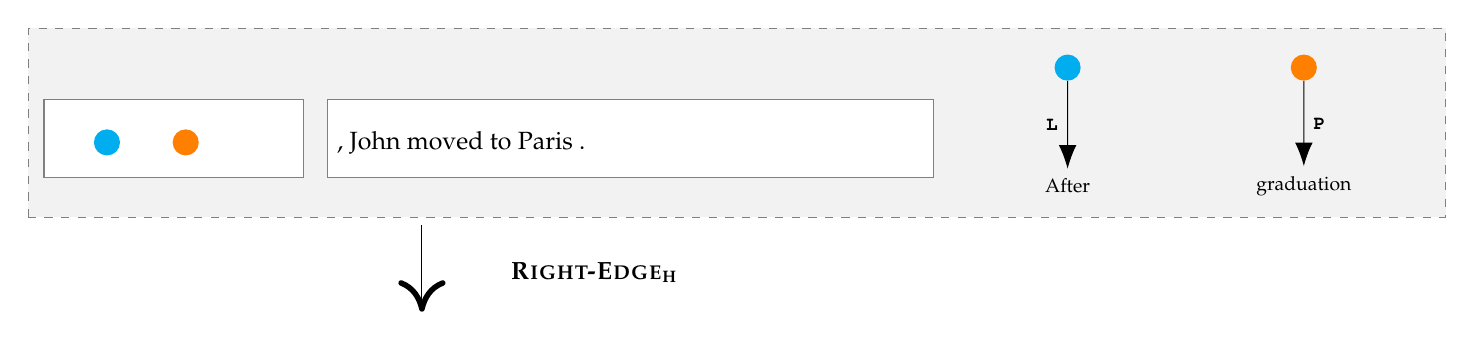
\begin{tikzpicture}[level distance=15mm, sibling distance=4cm, font=\small, -{Latex[length=3mm]}]
	\draw[color=gray,dashed,fill=lightgray!20] (0,-.5) rectangle (18,1.9);
	\draw[color=gray,fill=white] (0.2,0) rectangle (3.5,1);
	\node[fill=cyan, circle] at (1,.45) {};
	\node[fill=orange, circle] at (2,.45) {};
	\draw[color=gray,fill=white] (3.8,0) rectangle (11.5,1);
	\node[anchor=west] at (3.8,.45) {, John moved to Paris .};
	\node[fill=cyan, circle] at (13.2,1.4) {}
	  child {node[font=\scriptsize] {After} edge from parent node[font=\scriptsize\bf\ttfamily,left] {L}};
	\node[fill=orange, circle] at (16.2,1.4) {}
	  child {node[font=\scriptsize] {graduation} edge from parent node[font=\scriptsize\bf\ttfamily,right] {P}};
	\node[anchor=west] at (6,-1.2) {\bf\small\textsc{Right-Edge\textsubscript H}};
	\draw[arrows={->[line width=2pt,length=4mm,width=6mm]}] (5,-.6) -- (5,-1.7);
	\end{tikzpicture}
	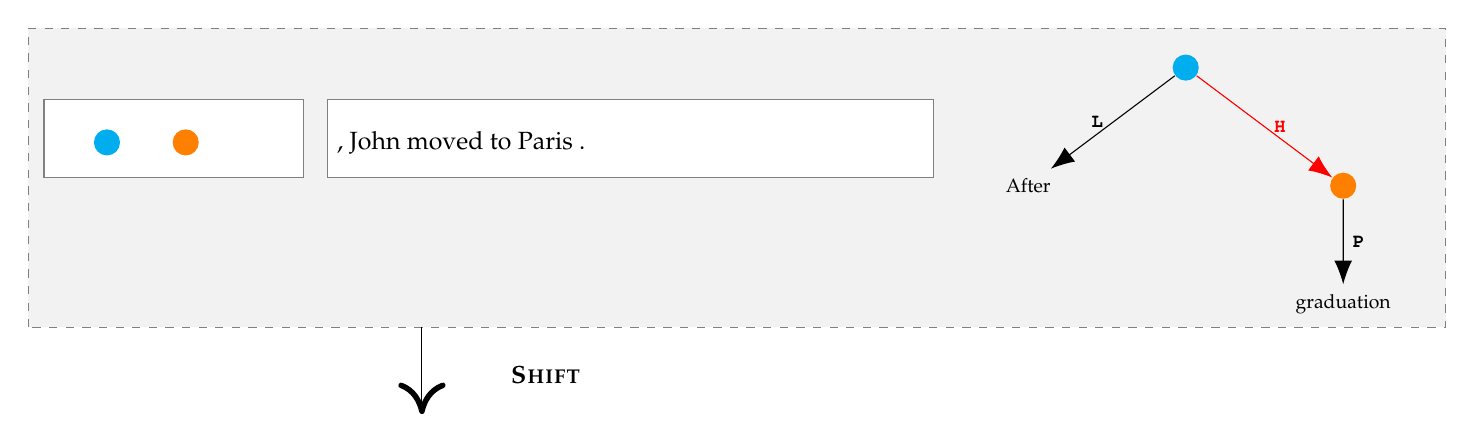
\begin{tikzpicture}[level distance=15mm, sibling distance=4cm, font=\small, -{Latex[length=3mm]}]
	\draw[color=gray,dashed,fill=lightgray!20] (0,-1.9) rectangle (18,1.9);
	\draw[color=gray,fill=white] (0.2,0) rectangle (3.5,1);
	\node[fill=cyan, circle] at (1,.45) {};
	\node[fill=orange, circle] at (2,.45) {};
	\draw[color=gray,fill=white] (3.8,0) rectangle (11.5,1);
	\node[anchor=west] at (3.8,.45) {, John moved to Paris .};
	\node[fill=cyan, circle] at (14.7,1.4) {}
	  child {node[font=\scriptsize] {After} edge from parent node[font=\scriptsize\bf\ttfamily,left] {L}}
	  child {node [fill=orange, circle] {}
	  {
	    child {node[font=\scriptsize] {graduation} edge from parent [black] node[font=\scriptsize\bf\ttfamily,right] {P}}
	  } edge from parent [red] node[font=\scriptsize\bf\ttfamily,right] {H} };
	\node[anchor=west] at (6,-2.5) {\bf\small\textsc{Shift}};
	\draw[arrows={->[line width=2pt,length=4mm,width=6mm]}] (5,-1.9) -- (5,-3);
	\end{tikzpicture}
	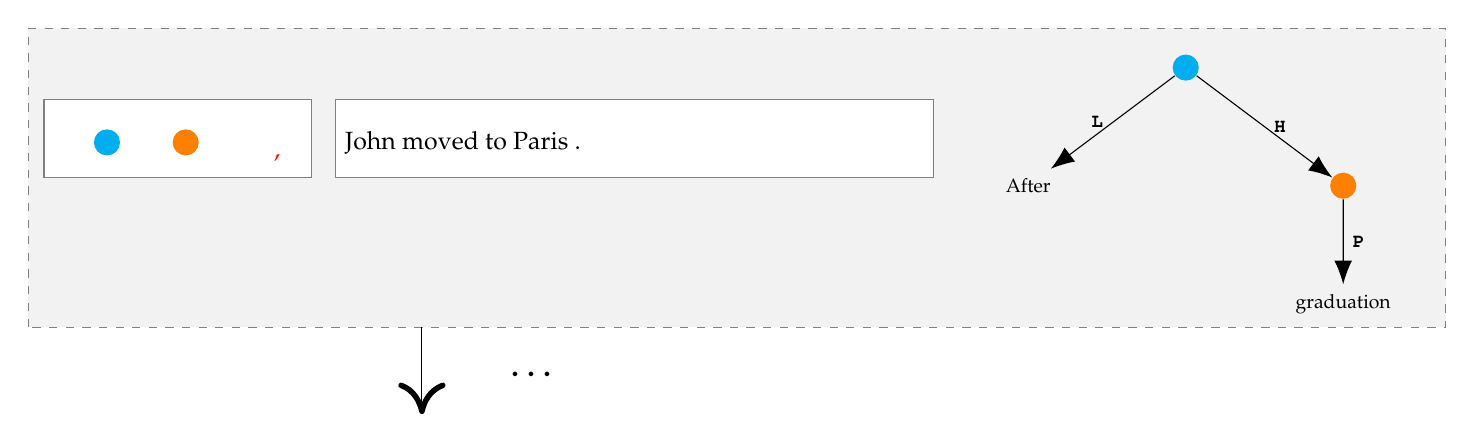
\begin{tikzpicture}[level distance=15mm, sibling distance=4cm, font=\small, -{Latex[length=3mm]}]
	\draw[color=gray,dashed,fill=lightgray!20] (0,-1.9) rectangle (18,1.9);
	\draw[color=gray,fill=white] (0.2,0) rectangle (3.6,1);
	\node[fill=cyan, circle] at (1,.45) {};
	\node[fill=orange, circle] at (2,.45) {};
	\node[color=red, anchor=west] at (3,.25) {,};
	\draw[color=gray,fill=white] (3.9,0) rectangle (11.5,1);
	\node[anchor=west] at (3.9,.45) {John moved to Paris .};
	\node[fill=cyan, circle] at (14.7,1.4) {}
	  child {node[font=\scriptsize] {After} edge from parent node[font=\scriptsize\bf\ttfamily,left] {L}}
	  child {node [fill=orange, circle] {}
	  {
	    child {node[font=\scriptsize] {graduation} edge from parent node[font=\scriptsize\bf\ttfamily,right] {P}}
	  } edge from parent node[font=\scriptsize\bf\ttfamily,right] {H} };
	\node[anchor=west] at (6,-2.5) {\Large \ldots};
	\draw[arrows={->[line width=2pt,length=4mm,width=6mm]}] (5,-1.9) -- (5,-3);
	\end{tikzpicture}
	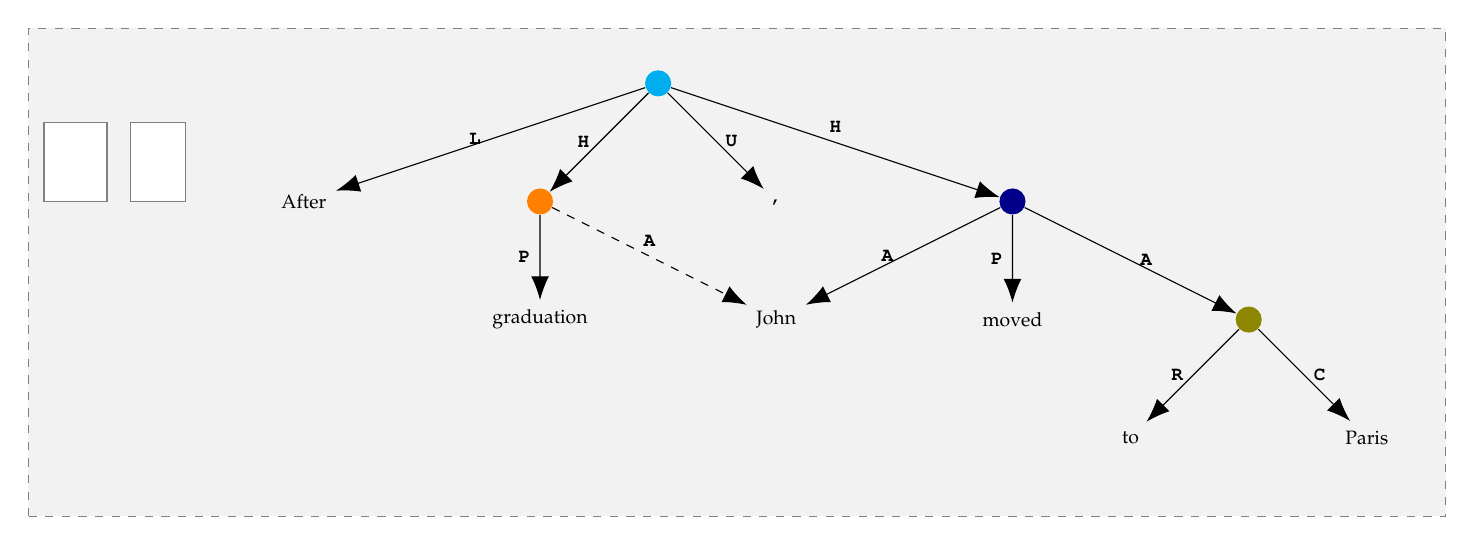
\begin{tikzpicture}[level distance=15mm, sibling distance=3cm, font=\small, -{Latex[length=3mm]}]
	\draw[color=gray,dashed,fill=lightgray!20] (0,-4) rectangle (18,2.2);
	\draw[color=gray,fill=white] (.2,0) rectangle (1,1);
	\draw[color=gray,fill=white] (1.3,0) rectangle (2,1);
    \node (ROOT) [fill=cyan,circle] at (8,1.5) {}
      child {node[font=\scriptsize] (After) {After} edge from parent node[font=\scriptsize\bf\ttfamily,left] {L}}
      child {node (graduation) [fill=orange,circle] {}
      {
        child {node[font=\scriptsize] {graduation} edge from parent node[font=\scriptsize\bf\ttfamily,left] {P}}
      } edge from parent node[font=\scriptsize\bf\ttfamily,left] {H} }
      child {node[font=\scriptsize\bf\ttfamily] {,} edge from parent node[font=\scriptsize\bf\ttfamily,right] {U}}
      child {node (moved) [fill=DarkBlue,circle] {}
      {
        child {node[font=\scriptsize] (John) {John} edge from parent node[font=\scriptsize\bf\ttfamily,left] {A}}
        child {node[font=\scriptsize] {moved} edge from parent node[font=\scriptsize\bf\ttfamily,left] {P}}
        child {node [fill=olive,circle] {}
        {
          child {node[font=\scriptsize] {to} edge from parent node[font=\scriptsize\bf\ttfamily,left] {R}}
          child {node[font=\scriptsize] {Paris} edge from parent node[font=\scriptsize\bf\ttfamily,right] {C}}
        } edge from parent node[font=\scriptsize\bf\ttfamily,right] {A} }
      } edge from parent node[font=\scriptsize\bf\ttfamily,above] {H} }
      ;
    \draw[dashed] (graduation) to node [font=\scriptsize\bf\ttfamily,above] {A} (John);
	\end{tikzpicture}
\end{minipage}
}

\vfill

\section*{Transition Classifier}

\begin{center}
   \vspace{-1mm}
   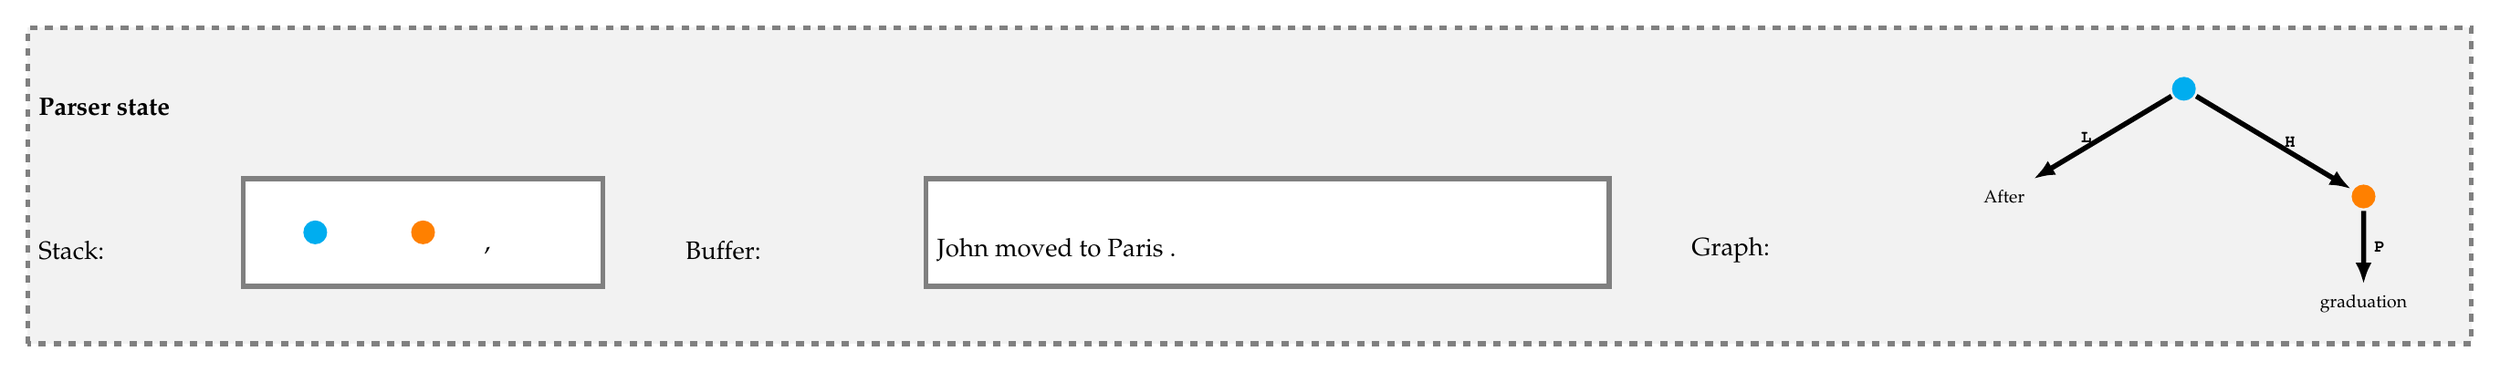
\begin{tikzpicture}[-{Latex[length=3mm]},level distance=15mm, sibling distance=5cm, line width=2pt]
   \draw[color=gray,dashed,fill=lightgray!20] (0,-.8) rectangle (34,3.6);
   \node[anchor=west] at (0,2.5) {\textbf{Parser state}};
   \node[anchor=west] at (0,.5) {Stack:};
   \draw[color=gray,fill=white] (3,0) rectangle (8,1.5);
   \node[fill=cyan, circle] at (4,.75) {};
   \node[fill=orange, circle] at (5.5,.75) {};
   \node[anchor=west] at (6.2,.5) {,};
   \node[anchor=west] at (9,.5) {Buffer:};
   \draw[color=gray,fill=white] (12.5,0) rectangle (22,1.5);
   \node[anchor=west] at (12.5,.5) {John moved to Paris .};
   \node[anchor=west] at (23,.5) {Graph:};
   \node[fill=cyan, circle] at (30,2.75) {}
     child {node[font=\scriptsize] {After} edge from parent node[font=\scriptsize\bf\ttfamily,left] {L}}
     child {node [fill=orange, circle] {}
     {
       child {node[font=\scriptsize] {graduation} edge from parent node[font=\scriptsize\bf\ttfamily,right] {P}}
     } edge from parent node[font=\scriptsize\bf\ttfamily,right] {H} };
   \end{tikzpicture}
   
   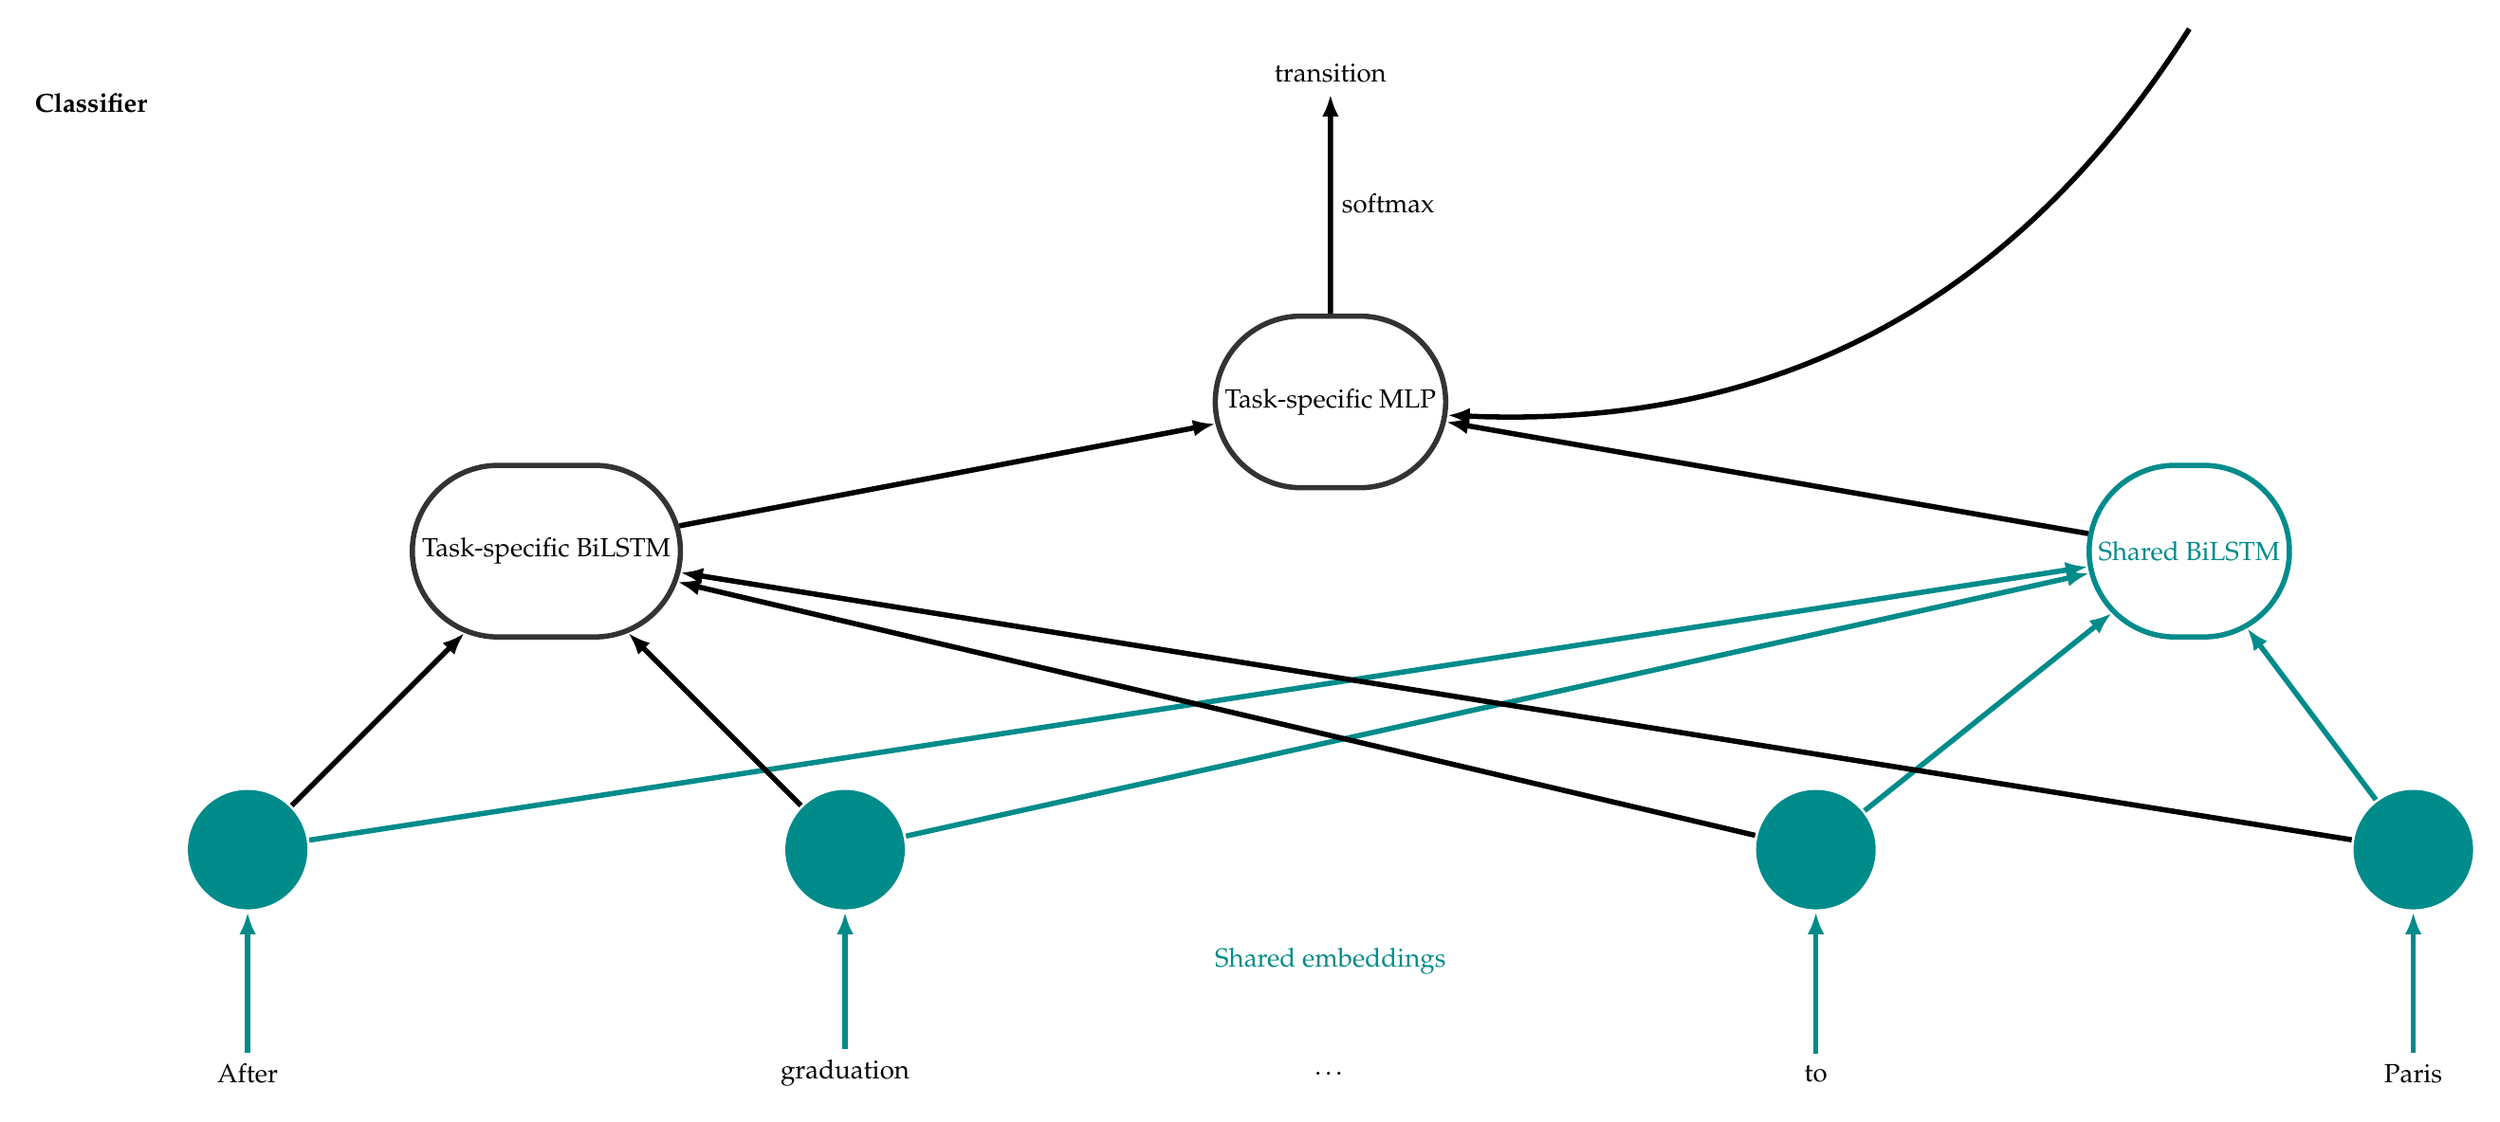
\begin{tikzpicture}[-{Latex[length=3mm]},thick, line width=2pt]
   \node[anchor=west] at (-7,16) {\textbf{Classifier}};
   \tikzstyle{main}=[rounded rectangle, minimum size=23mm, draw=black!80, node distance=12mm]
   \node[main] (specific) at (0,10) {Task-specific BiLSTM};
   \node[main,color=DarkCyan] (shared) at (22,10) {Shared BiLSTM};
   \node[color=DarkCyan] (embeddings) at (10.5,4.5) {Shared embeddings};
   \foreach \i/\word in {-4/{After},4/{graduation},17/{to},25/{Paris}} {
       \node (x\i) at (\i,3) {\word};
       \node[main, minimum size=16mm, fill=DarkCyan, draw=none] (e\i) at (\i,6) {};
       \path[color=DarkCyan] (x\i) edge (e\i);
       \path (e\i) edge (specific);
       \path[color=DarkCyan] (e\i) edge (shared);
   }
    \node (x4) at (10.5,3) {\ldots};
    \node[main] (mlp) at (10.5,12) {Task-specific MLP};
    \path (specific) edge (mlp);
    \path (shared) edge (mlp);
    \coordinate (state) at (22,17);
    \path (state) edge [bend left] (mlp);
    \node (transition) at (10.5,16.4) {transition};
    \path (mlp) edge node[right] {softmax} (transition);
   \end{tikzpicture}
\end{center}


\hrule

\section*{Unified DAG Format}

We convert UD into a format similar to UCCA and
supported by TUPA.

\begin{center}
  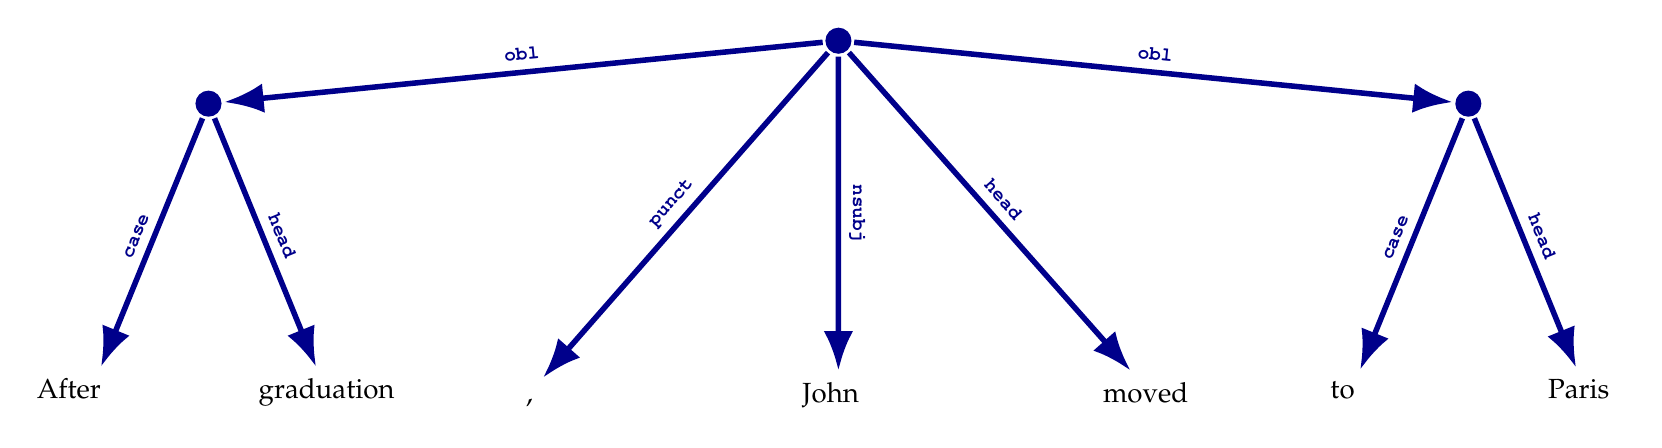
\begin{tikzpicture}[-{Latex[length=5mm]}, color=DarkBlue, line width=2pt,
      every node/.append style={sloped,anchor=south,auto=false,font=\scriptsize\bf\ttfamily},
      level 1/.style={sibling distance=4cm,level distance=1cm},
      level 2/.style={sibling distance=3cm,level distance=4cm}]
    \tikzstyle{word} = [font=\rmfamily,color=black]
    \node (ROOT) [fill=DarkBlue,circle] {}
      child {node (after) [fill=DarkBlue,circle] {}
      {
        child {node [word] {After{\color{white}g}\quad\quad} edge from parent node {case}}
        child {node [word] {\quad graduation\quad\quad} edge from parent node {head}}
      } edge from parent node {obl}}
      child {node {}
      {
        child {node [word] (comma) {\quad,{\color{white}g}} edge from parent [draw=none]}
      } edge from parent [draw=none]}
      child {node {}
      {
        child {node [word] (John) {John{\color{white}g}} edge from parent [draw=none]}
      } edge from parent [draw=none]}
      child {node {}
      {
        child {node [word] (moved) {moved{\color{white}g}} edge from parent [draw=none]}
      } edge from parent [draw=none]}
      child {node (to) [fill=DarkBlue,circle] {}
      {
          child {node [word] {to{\color{white}g}} edge from parent node {case}}
          child {node [word] {Paris{\color{white}g}} edge from parent node {head}}
      } edge from parent node {obl}}
      ;
      \draw (ROOT) to node {punct} (comma);
      \draw (ROOT) to node {nsubj} (John);
      \draw (ROOT) to node {head} (moved);
  \end{tikzpicture}
  \captionof{figure}{\color{DarkBlue} Converted UD.}
\end{center}

\hrule



\section*{Results}



\begin{multicols}{2}
\color{DarkSlateGray}
\tiny\titleformat*{\section}{\small}
\bibliographystyle{plain}
\bibliography{references}

\color{Black}
\begin{adjustbox}{margin=3mm,frame,minipage=\columnwidth}
\centering\large
Please join SemEval 2019 Task 1: \\
Cross-lingual Semantic Parsing with UCCA

\begin{minipage}{.3\textwidth}
\includegraphics[width=\textwidth]{qr}\end{minipage}
\hfill
\begin{minipage}{.6\textwidth}\Large\url{tinyurl.com/semeval-ucca}\end{minipage}
\end{adjustbox}
\end{multicols}

\end{multicols}
\end{document}
